\documentclass[12pt,american]{article}
\usepackage[T1]{fontenc}
\usepackage[latin9]{inputenc}
\usepackage[letterpaper]{geometry}
\geometry{verbose,tmargin=1in,bmargin=1in,lmargin=1in,rmargin=1in}
\usepackage{textcomp}
\usepackage{amstext}
\usepackage{amssymb}
\usepackage{amsmath}
\usepackage{babel}
\usepackage{hyperref}
\usepackage{tcolorbox}
\usepackage{wrapfig} 

%---------------------------------------------------------
%  Toggle to label equations 
%
\def \plabel#1 {\label{#1} }
% \def \plabel#1 {\label{#1} \qquad{#1} }
%
%---------------------------------------------------------
\def\beq{\begin{equation}}
\def\eeq{\end{equation}}
\def\bea{\begin{eqnarray}}
\def\eea{\end{eqnarray}}
\def \be{\mbox{\boldmath{$e$}}}
\def \u{\mbox{\boldmath{$u$}}}
\def \v{\mbox{\boldmath{$v$}}}
\def \bx{\mbox{\boldmath{$x$}}}
\def \ep{\epsilon}
\def \bep{\mbox{\boldmath{$\epsilon$}}}
\def \be{\mbox{\boldmath{$e$}}}
\def \bs{\mbox{\boldmath{$s$}}}
\def \bsig{\mbox{\boldmath{$\sigma$}}}
\def \barsig{\mbox{{$\overline\sigma$}}}
\def \barep{\mbox{{$\overline{\ep}$}}}
\def \sigo{\sigma_{o}}
\def \pie{\Pi_{Elastic}}
\def \pit{\Pi_{Total}}
\def \cS{{\cal{S}}}
\def \cV{{\cal{V}}}
\def \us{{u^{*}}}
\def \xs{{x^{*}}}
\def \bxs{{\bx^{*}}}
\def \J{\mbox{\boldmath{$J_n$}}}
\def \bF{\mbox{\boldmath{$F$}}}
\begin{document}
\title{Nonlinear elastic rod}
\author{Andre, Paul, Elise}
\date{\today}
\maketitle
\tableofcontents
\newpage
\section{Introduction}
We derive equations of equilibrium for uniaxial deformation of an elastic rod.  
We approach the problem from three perspectives:  strong form (direct equilibrium equation), weak form, 
and minimization of 
the total potential energy.  
We eventually consider the material behavior of the rod as nonlinear, but assume the strains 
are sufficiently small to neglect geometric nonlinearity.  To begin with, however, 
we start with linear elastic material assumption. 
\section{Strong formulation}
\subsection{Fundamental equations}
Here we let $u(x)$ represent the axial displacement of a particle whose initial position is $x$, 
$\ep(x)$ is the axial strain in the rod at location $x$, and $\sigma(x)$ is the stress acting on the 
cross section of the rod at 
location $x$.  $f(x)$ is a body force (i.e.\ a force per unit volume) assumed to be known in the rod.  
Here we focus on the special case that the rod has uniform cross sectional area, $A$, and zero traction along 
its length.  
\bigskip
\noindent
{\em Equilibrium equation:}
\beq
\frac{d\sigma}{dx}  + f = 0 
\plabel{equil}
\eeq
%{\em Linear constitutive equation:}
%\beq
%\sigma = E \epsilon
%\plabel{linear-sig-ep}
%\eeq
{\em Constitutive equation:}
\beq
\sigma = \Sigma(\ep) = E \ep 
\plabel{sig-ep}
\eeq
{\em Kinematics equation:}
\beq
\ep = \frac{d u}{dx} 
\plabel{u-ep}
\eeq
\begin{tcolorbox}[title= Exercise]
Derive equation (\ref{equil}). 
\end{tcolorbox}
\subsection{An example $1D$ boundary value problem} 
We now consider a rod that has length $L$.  It is fixed at $x=0$ and is acted upon at $x=L$ by a force $P$.  
We let $\sigo = P/A$.   A body force $f(x)$ is known.    Therefore, in addition to equations (\ref{equil}-\ref{u-ep}), 
we need to add the boundary conditions: 
\bea
u(0) &=& u_o
\plabel{bc1} \\ 
\sigma(L) &=& P/A = \sigo .
\plabel{bc2}
\eea 
\begin{tcolorbox}[title= Strong Form 1]{
% \fbox{
Given $u_o$, $\sigo$, $E$,  and $f(x)$,  for $0 < x < L$, 
find 
$u(x)$, $\ep(x)$, $\sigma(x)$ that satisfy:
\bea
\frac{d\sigma}{dx}  + f &=& 0 \\  
\sigma &=& E \ep \\ 
\ep &=& \frac{d u}{dx} \\
u(0) &=& u_o \\ 
\sigma(L) &=& \sigo .
\eea 
}
\end{tcolorbox}
This box summarizes all our fundamental equations and boundary conditions.  The unknowns are $u, \ep, \sigma$.  
To solve for these unknowns, we have two first-order odes, and one algebraic equation (\ref{sig-ep}).  
If we were to set about to solving this problem, the first thing that we might do is use equations (\ref{sig-ep}) 
and (\ref{u-ep}) to eliminate the unknowns $\sigma$ and $\ep$ in favor of $u(x)$.  This would then give us: 
\begin{tcolorbox}[title= Strong Form 2]{
% \fbox{
Given $u_o$, $\sigo$, $E$, and $f(x)$,  for $0 < x < L$, 
find 
$u(x)$, that satisfies:
\bea
\frac{d}{dx} \left(E \frac{du}{dx} \right) + f &=& 0
\plabel{11} \\  
%\sigma &=& \Sigma(\ep) \\ 
%\ep &=& \frac{d u}{dx} \\
u(0) &=& u_o 
\plabel{12} \\  
\left. E \frac{du}{dx} \right|_{x=L} &=& \sigo .
\plabel{13} 
\eea 
}
\end{tcolorbox}
Here we have just the one unknown function, $u(x)$ and one differential equation.  
These problems are equivalent, but they are different.  
One has three unknown functions; the other one unknown function.
One has two first order differential equations; the other had one second order differential equation. 
One yields all quantities of potential interest (i.e. $u, \ep, \sigma$); the other yields only $u$.  
If one uses the Strong Form 2 and wishes to know the stress, then the stress must be computed as a 
{\em post-process}.  Generally speaking, if one knows any of the functions, $u, \ep, \sigma$, then 
the problem is considered to be solved.  The others can be evaluated {\em relatively} 
easily from (\ref{sig-ep}) and/or (\ref{u-ep}).  
\section{Minimum potential energy}
Here we reformulate the problem using the principle of minimum potential energy.  
\subsection{Fundamental equations} 
\subsubsection{Stored elastic potential energy}
Let $W$ denote the elastic energy density, i.e.\ the energy per unit volume, contained in a deformed solid.  
(Normally we think of $W = W(\ep)$ to be a pure function of strain (i.e.\ it depends {\em only} on strain).  
One definition of an elastic material is that $W = W(\ep)$.)  For a linear elastic material in 
uniaxial tension, $W = \frac{1}{2} E \ep^2$. 
\bigskip
\noindent
{\em Elastic potential energy:}
\bea
\pie[u] &=& \int_V W(\ep(u)) dV  \\ 
	&=& \int_0^L W(\ep(u)) A\, dx 
\plabel{pie}
\eea
Note that in (\ref{pie}), we think of $\ep$ as determined by $u(x)$ through equation (\ref{u-ep}).  
\subsubsection{Work done by loading} 
The sum of all work done by all externally applied loads is: 
\bigskip
\noindent
{\em External work:}
\bea
\ell[u] &=& \int_V f(x) \cdot u(x) dV  + P \cdot u(L)  \\
	&=& \int_0^L f(x) \cdot u(x) A\, dx  + P \cdot u(L) 
\plabel{ell}
\eea
Again, 
Note that here $V = (0,L) \times A$, and $dV = A\, dx$. 
The work done by these loads comes at the loss of some energy.  We shall assume that this work 
represents energy lost by some conservative loading machine, so that 
\beq
\Pi_{Load}[u] = - \ell[u]. 
\eeq
That is, work done on the rod is the energy lost by $\Pi_{Load}$.  
\subsubsection{Total potential energy}
The total potential energy is, therefore, $\pit = \pie + \Pi_{Load}$, or 
\bigskip
\noindent
{\em Total potential energy:}  
\bea
\pit[u] &=& \pie[u] - \ell[u] \\ 
	&=& \int_0^L W(\ep(u))  - f(x) \cdot u(x) A\, dx  - P \cdot u(L) 
\eea
\subsection{Principle of minimum potential energy} 
\begin{tcolorbox}[title= Principle of minimum potential energy - wordy]
Of all admissible functions, $u(x)$, the equilibrium 
displacement field is given by the $u(x)$ that minimizes $\pit[u]$.
\end{tcolorbox}
\subsubsection{Admissible displacement fields} 
Admissible displacement fields must satisfy an appropriate degree of continuity and 
satisfy our {\em essential} boundary conditions.  In our example boundary value 
problem, the essential boundary condition is (\ref{bc1}).  The appropriate degree of 
continuity in $1D$ is that the functions be at least continuous.  
% An alternative way 
% of prescribing that the function, $u(x)$ be continuous in $1D$ is to require: 
% \beq
% \int_0^L \left(\frac{du}{dx}\right)^2 \dx < \infty. 
% \eeq
The set of continuous functions defined for $0 \le x \le L$ 
is denoted $C^0[0,L]$.  
To say that 
$u(x)$ is continuous is equivalent to saying that 
$u(x)$ is in the set $C^0$, or in math-speak, $u(x) \in C^0[0,L]$. 
\footnote{The superscript $0$ indicates how many derivatives of 
$u(x)$ are required to be continuous.  Thus $C^3[0,L]$ is the set of all functions 
whose third derivative (and therefore second and first and zeroth) 
is continuous between $0 \le x \le L$.}
Therefore we introduce the set $\cS$ of admissible displacement fields, $u(x)$: 
\beq
\cS = \left\{ u(x) | u(x)\in C^0[0,L];\  u(0) = u_o. \right\}
\plabel{S}
\eeq
This reads, ``$\cS$ is the set of all $u(x)$ such that $u(x)$ is continuous and $u(0) = 0$.''
\begin{tcolorbox}[title= Principle of minimum potential energy - mathy]
The equilibrium displacement field, $\us$, is the minimizer over all 
$u(x) \in \cS$ of: 
\bea 
\pit[u] &=& \int_0^L \frac{1}{2} E \left(\frac{du}{dx} \right)^2  - f(x) \cdot u(x) A\, dx  - P \cdot u(L),  
\plabel{pit}
\\ 
\mbox{where} \qquad 
\cS &=& \left\{ u(x) | u(x)\in C^0[0,L];\  u(0) = u_o. \right\}
\eea
\end{tcolorbox}
\subsubsection{Admissible variation fields} 
Pick any $u(x) \in \cS$.  Then $v(x)$ is an {\em admissible variation} 
if (and only if) $u(x) + v(x) \in \cS$.  We let $\cV$ denote the set of all 
admissible variations.  
\begin{tcolorbox}[title=Exercise:]
Use the definition given to show that 
\beq
\cV = \left\{ v(x) | v(x)\in C^0[0,L];\  v(0) = 0. \right\}
\plabel{V}
\eeq
\end{tcolorbox}
\subsection{Euler Lagrange Equations:  The connection between the strong form 
and the principle of minimum potential energy} 
We let $\us\in \cS$ denote the minimizer of $\pit[u]$.  
Our goal here is to show that $\us$ satisfies Strong Form 2.  
We begin by choosing an arbitrary function $v(x) \in \cV$.  
Once we pick that function, it's picked.  It doesn't change.  
To say that it's arbitrary means that it doesn't matter which one we pick, 
but we have to pick one.  In this example, we can imagine it's $v(x) = 8x$.  
We next define the function $F(\alpha)$, where $\alpha$ is an arbitrary 
scalar, and 
\beq
F(\alpha) = \pit[\us + \alpha v]. 
\plabel{100}
\eeq
We note that since $\us$ minimizes $\pit[u]$, 
then $F(\alpha)$ is minimum at $\alpha = 0$: 
\beq
F(\alpha) = \pit[\us + \alpha v] \ge \pit[\us ]  = F(0). 
\plabel{101}
\eeq
Since $\alpha =0$ is a minimum of $F(\alpha)$, then the slope of $F$ is zero at that 
point.  Hence 
$\left.\frac{dF}{d\alpha}\right|_{\alpha = 0} = 0$.  Computing gives us: 
\bea
\left.\frac{dF}{d\alpha}\right|_{\alpha = 0} 
 	&=&
\left.\frac{d}{d\alpha}\right|_{\alpha = 0} 
\int_0^L \frac{1}{2} E 
\left(\frac{d\us}{dx}  
+ \alpha \frac{dv}{dx}  \right)^2  
- f(x) \cdot (\us + \alpha v(x)) A\, dx  
% \nonumber \\
% && \qquad \qquad 
- P \cdot (u(L) + \alpha v(L))
\nonumber \\
 	&=&
\left.\left\{ 
\int_0^L E 
\left(\frac{d\us}{dx}  
+ \alpha \frac{dv}{dx}  \right) 
\frac{dv}{dx}  
- f(x) \cdot (v(x)) A\, dx  - P \cdot (v(L))
\right\}
\right|_{\alpha = 0} 
\\
 	&=&
\int_0^L E 
% \left(
\frac{d\us}{dx}  
 % \right) 
\frac{dv}{dx}  
- f(x) \cdot v(x) A\, dx  - P \cdot v(L)
\plabel{102} \\ 
 	&=& 0 \qquad \forall v(x) \in \cV 
\plabel{103}
\eea
To see the connection between (\ref{102}) and (\ref{11}), 
we use integration by parts on the first term in (\ref{102}).  
Integration by parts is really the product rule of differentiation backwards. 
Remembering this helps when applying it in multi-dimensional contexts.  
Therefore, in order to integrate (\ref{102}) by parts, we first rewrite 
the product of derivatives using the product rule: 
\beq
\frac{d}{dx}  \left( E \frac{d\us}{dx}  v(x) \right) 
% &=& 
=
E \frac{d\us}{dx}  
\frac{dv}{dx}  
+ 
v(x) \frac{d}{dx}  \left( E \frac{d\us}{dx}  \right)
\eeq
Therefore, 
\bea
\int_0^L
\frac{d\us}{dx}  
\frac{dv}{dx}  
A\, dx  
 	&=& 
\int_0^L
\frac{d}{dx}  \left( E \frac{d\us}{dx}  v(x) \right) 
- 
v(x) \frac{d}{dx}  \left( E \frac{d\us}{dx}  \right)
A\, dx  
\\
 	&=& 
\int_0^L
\frac{d}{dx}  \left( E \frac{d\us}{dx}  v(x) \right) 
A\, dx  
- 
\int_0^L
v(x) \frac{d}{dx}  \left( E \frac{d\us}{dx}  \right)
A\, dx  
\\
 	&=& 
\left.\left( E \frac{d\us}{dx}  v(x) \right) 
A\right|_{x=0}^{x=L} 
- 
\int_0^L
v(x) \frac{d}{dx}  \left( E \frac{d\us}{dx}  \right)
A\, dx  
\\
\mbox{since\ $v \in \cV$:} \qquad  	&=& 
\left.\left( E \frac{d\us}{dx}
\right) A \right|_{x=L} 
  v(L) 
- 
\int_0^L
v(x) \frac{d}{dx}  \left( E \frac{d\us}{dx}  \right)
A\, dx  
\plabel{104}
\eea
\begin{tcolorbox}[title= Exercise]
Get (\ref{104}) from the line above.  When you know how to do it, it's one line.  
\end{tcolorbox}
We now use (\ref{104}) to rewrite equation (\ref{102}) in the form: 
\beq
- \int_0^L 
v(x) 
\left[
\frac{d}{dx}  \left( E \frac{d\us}{dx}  \right)
+ f(x) \right] A\, dx  
+\left[ \left.\left( E \frac{d\us}{dx}
\right) \right|_{x=L} A
- P \right] v(L)
 	= 0 \qquad \forall v(x) \in \cV 
\plabel{105}
\eeq
Since (\ref{105}) holds for any choice of $v(x) \in \cV$, then we can conclude:
\bea
\frac{d}{dx}  \left( E \frac{d\us}{dx}  \right) + f(x)  
&=& 0 
\plabel{106} \\ 
\left.\left( E \frac{d\us}{dx}
\right) \right|_{x=L} A
&=& P . 
\plabel{107} 
\eea
Equations (\ref{106}) and (\ref{107}) are the Euler-Lagrange equations resulting from 
minimizing the functional $\pit[u]$.  
We see that $\us(x)$ 
satisfies differential equation (\ref{106}), which is the same differential 
equation as (\ref{11}).  Furthermore, $\us(x)$ satisfies boundary condition 
(\ref{107}), which is the same boundary condition as (\ref{13}).  
Since $\us(x)$ is required to be in the set $\cS$, then $\us$ also satisfies (\ref{12}).  
Therefore $\us$ satisfies equations (\ref{11}, \ref{12}, \ref{13}) of Strong Form 2.  
Since the solution of Strong Form 2 is unique, then its solution also minimizes 
$\pit[u]$ over all functions in $\cS$.  
In the process of minimizing $\pi[u]$, we found that boundary condition 
(\ref{107}) (or (\ref{13})) resulted naturally as a consequence of the minimization.  By contrast, 
boundary condition (\ref{12}) is an essential part of the formulation of the minimization problem. 
Without boundary condition (\ref{12}), the minimization problem wouldn't make sense; there would be 
no minimum.  Therefore, (\ref{12}) is called an {\em essential boundary condition}, while (\ref{13}) 
is called a {\em natural boundary condition}. 
\begin{tcolorbox}[title= Summary] 
The function $\us(x)\in \cS$ minimizes the total potential energy $\pit[u]$, compared to all 
other functions in $\cS$.  The minimizing function $\us$ 
satisfies equations (\ref{11}, \ref{12}, \ref{13}) of Strong Form 2, 
and likewise, the solution of Strong Form 2 minimizes 
$\pit[u]$. 
\end{tcolorbox}
\section{Weak formulation}
\subsection{Obtained from minimum potential energy}
Above we showed that Strong Form 2 follows from equation (\ref{102}).  
We divide (\ref{102}) through by the constant area $A$ and write that result here 
for convenience: 
\beq
\int_0^L E 
\frac{d\us}{dx}  
\frac{dv}{dx}  
- f(x) \cdot v(x) \, dx  - \sigo \cdot v(L)
 	= 0 \qquad \forall v(x) \in \cV 
\plabel{weak1}
\eeq
Equation (\ref{weak1}) is known as the weak form the boundary value problem.  More precisely, 
the weak form of the boundary value problem is:  
\begin{tcolorbox}[title= Weak Form] 
Given $u_o$, $\sigo$, $E$,  and $f(x)$,  for $0 < x < L$, 
find $u(x) \in \cS$ such that for all $v(x) \in \cV$, 
\beq
\int_0^L E 
\frac{d\us}{dx}  
\frac{dv}{dx}  
- f(x) \cdot v(x) \, dx  - \sigo \cdot v(L)
 	= 0 
\plabel{weak}
\eeq
\end{tcolorbox}
\subsection{Derivation from Strong Form 2}
\begin{tcolorbox}[title= Exercise: Derive the weak form from the strong form] 
Let $v \in \cV$.  Compute $\int_0^L (\ref{11})\,  v(x) dx$.  
Integrate by parts and simplify to derive (\ref{weak}).  
In the process of getting (\ref{weak}), you will need to use (\ref{12}) and (\ref{13}) 
various steps.  Since you use (\ref{11}, \ref{12}, \ref{13}), this implies that the 
solution of Strong Form 2 also satisfies Weak Form for $\u \in \cS$.  
Can you identify where each of these eqns is used? 
(\ref{12}) is subtle.
\end{tcolorbox}
Let's first express $\int_0^L(\ref{11})v(x)dx$ using ($\ref{11}$):
\beq
\int_0^L \left[ \frac{d}{dx} \left( E \frac{du}{dx} \right) v(x) + f(x)v(x) \right]dx = 0
\eeq
{\em Evaluate chain rule:}
\bea
\frac{d}{dx} \left( E \frac{du}{dx} v(x) \right) &=&
\frac{d}{dx} \left( E \frac{du}{dx} \right) v(x) +
E \frac{du}{dx} \frac{dv}{dx} \\
\frac{d}{dx} \left( E \frac{du}{dx} \right) v(x) &=&
\frac{d}{dx} \left( E \frac{du}{dx} v(x) \right) -
E \frac{du}{dx} \frac{dv}{dx}
\eea
\beq
\int_0^L \frac{d}{dx} \left( E \frac{du}{dx} v(x) \right) - E \frac{du}{dx} \frac{dv}{dx} + fv(x) dx = 0
\eeq
{\em Evaluate the following integral:}
\beq
\int_0^L \frac{d}{dx} \left( E \frac{du}{dx} v(x) \right) = \left. \left( E \frac{du}{dx} v(x) \right) \right]_{x=0}^{x=L} = 
\left( \left. E \frac{du}{dx} \right]_{x=L} v(L) \right) - 
\left( \left. E \frac{du}{dx} \right]_{x=0} v(0) \right)
\eeq
\beq
\left( \left. E \frac{du}{dx} \right]_{x=L} v(L) \right) - 
\left( \left. E \frac{du}{dx} \right]_{x=0} v(0) \right) - 
\int_0^L \left[ E \frac{du}{dx} \frac{dv}{dx} - fv(x) \right] dx = 0
\eeq
{\em The first term can be simplified using ($\ref{13}$):}
\beq
\left( \left. E \frac{du}{dx} \right]_{x=L} v(L) \right) = 
\sigo \cdot v(L)
\eeq
{\em Our essential boundary condition is defined in ($\ref{12}$). This information helps us simplify the second term in (45) since $v(x)$ must be 0 at all points defined by ($\ref{12}$) $\therefore$ $v(0) = 0$ as articulated in (24)}
\beq
v(0) = 0 \therefore \left( \left. E \frac{du}{dx} \right]_{x=0} v(0) \right) = 0
\eeq
{\em Finally,}
\beq
\sigo \cdot v(L) - \int_0^L \left[ E \frac{du}{dx} \frac{dv}{dx} - fv(x) \right] dx = 0
\eeq
{\em Rewriting slightly, we can see the same form presented in ($\ref{weak}$):}
\beq
\int_0^L E \frac{du}{dx} \frac{dv}{dx} - 
f(x) \cdot v(x) dx -
\sigo \cdot v(L) = 0
\eeq
\section{A mixed weak form}
\subsection{Derivation from Strong Form 1}
\subsection{Derivation from a mixed variational principle}
\section{Non-linear Weak Form}
Here we will explore an example in which we consider the material behavior of the rod as nonlinear, as defined below:
\\
{\em Constitutive relationship:}
\beq
\sigma = E \epsilon e^{\beta \epsilon}
\plabel{50}
\eeq
\begin{tcolorbox}[title= Nonlinear Strong Form]
Given $u_0$, $ \sigma_0 $, $E$, and $f(x)$, for $0<x<L$, find $u(x)$, $\epsilon(x)$,$\sigma(x)$ that satisfy:
\beq
\frac{d}{dx} \left( E \frac{du}{dx} e^{\beta \frac{du}{dx}} \right) + f = 0
\eeq
\beq
u(0) = u_0
\eeq
\beq
\left. E\frac{du}{dx} \right|_{x=L} = \sigo
\eeq
\end{tcolorbox}
\beq
\int_0^L \sigma(\epsilon) \frac{dv}{dx} - fvdx - P v(L) = 0
\eeq
\beq
\int_0^L EA \frac{du}{dx} e^{\beta \frac{dv}{dx}} \frac{dv}{dx} - fvdx - P v(L) = 0
\plabel{nlwf}
\eeq
{\em Linear shape function:}
\beq 
N(x) = \begin{bmatrix} 1-\frac{x}{L} & \frac{x}{L} \end{bmatrix} ;
B = \frac{dN}{dx} = \begin{bmatrix} \frac{L-1}{L} & \frac{1}{L} \end{bmatrix}
\eeq 
\subsection{Single Finite Element Approximation}
\beq
u(x) \approx U_1N_1(x) + U_2N_2(x)
\eeq
\beq
v(x) \approx V_1N_1(x) + V_2N_2(x)
\eeq
\beq 
N_1(x) = \frac{L-x}{L};
N_2(x) = \frac{x}{L};
B_2 = \frac{1}{L}
\eeq 
\beq 
\int_0^L \left[ EAU_2B_2e^{\beta U_2B_2}V_2B_2 - f V_2N_2 \right] dx - P V_2 N(L)
\eeq 
{\em Solve integral and simplify:}
\beq 
AEL \frac{U_2}{L^2}e^{\beta U_2 /L} = P
\eeq  
Newton's method will be used to solve for $U_2$
\beq
F(U_2) = AEL \frac{U_2}{L^2}e^{\beta U_2 /L} - P = 0
\eeq
{\em First guess:}
\beq
U_2 = U_2^{(0)} = 0
\plabel{newt-guess}
\eeq
{\em Approximate $F(U_2)$ using first guess $(U_2^{(0)})$}
\beq
F(U_2) = F(U_2^{(0)} + \delta U_2)
\eeq
{\em Using a first-order Taylor Series expansion, (\ref{newt-guess}) can be rewritten as such:}
\beq
F(U_2) \approx F(U_2^{(0)}) + \frac{dF}{dU}\delta U_2
\eeq
\beq 
F'(U) = \frac{AE}{L} e^{\beta U/L} \left( 1 + U\frac{\beta}{L}\right)
\eeq 
{\em At $U=0$ (our first approximation is analogous to linear elastic deformation):}
\beq 
F'(0) = \frac{AE}{L} \therefore \delta U = \frac{PL}{AE}
\eeq 
{\em For the next Newton iteration (using $\delta U$ as our guess) :}
\beq 
F'(U^{(1)} = P \left( e^{\beta P/AE} -1 \right)
\eeq 
\beq 
F'(U^{(1)} + \left. \frac{dF}{dU} \right|_{U^{(1)}} \delta U = 0
\eeq 
\beq 
P \left( e^{\beta P/AE} -1 \right) + \frac{AE^*}{L} \delta U = 0
\eeq 
{\em where $E^* = E e^{\beta P/AE} \left( 1 + \frac{\beta P}{AE} \right)$. This result is analogous to the first (linear elastic) Newton iteration, with an "updated" modulus. This modulus ($E^*$) is representative of the nonlinear behavior of the material. In this case, the modulus is a function of the applied load and varies with the displacement (strain).}
\beq 
\delta U = \frac{-PL}{AE^*} \left( e^{\beta P/AE} - 1 \right)
\eeq 
\subsection{Finite Element Approximation (2 elements)}
Next, let's consider the same nonlinear elastic rod solved with two finite elements. The weak form can be restated from (\ref{nlwf}):
\begin{tcolorbox}[title= Nonlinear Weak Form]{
% \fbox{
Given $u_o$, $\sigo$, $E$, $\beta$,  and $f(x)$,  for $0 < x < L$, 
find $u^* \in \cS$ such that for all $v(x) \in \cV$, 
\beq
\int_0^L \left[
E \frac{du^*}{dx} e^{\beta \frac{du^*}{dx}} \frac{dv}{dx} - 
f(x) \cdot v(x)
\right] dx - \sigo \cdot v(L) = 0
\plabel{nlweak}
\eeq
}
\end{tcolorbox}
\beq 
u(x) \approx U_0N_0(x) + U_1N_1(x) + U_2N_2(x)
\eeq 
\beq 
v(x) \approx V_0N_0(x) + V_1N_1(x) + V_2N_2(x)
\eeq 
{\em Impose essential boundary conditions:}
\beq 
u(0) \approx U_0 = 0; v(0) \approx V_0 = 0
\eeq 
\beq 
u(x) \approx U_1N_1(x) + U_2N_2(x); v(x) \approx V_1N_1(x) + V_2N_2(x)
\eeq 
\beq 
\sum_{elms} \int_{L_e} \left[ EA \frac{du}{dx} e^{\beta \frac{du}{dx}} \frac{dv}{dx} - fv(x) \right] dx - Pv(L)
\eeq 
{\em Assume no body forces ($f=0$)}
\begin{align*}
\int_0^{h_1} \left[ EA \left(U_1B_1 \right) e^{\beta \left(U_1B_1 \right)} V_1B_1 \right] dx
\\
+ \int_0^{h_2} \left[ EA \left(U_1B_1 +U_2B_2 \right) e^{\beta \left(U_1B_1 + U_2B_2\right)} \left( V_1B_1 + V_2 B_2 \right) \right] dx - P \left[ V_1N_1(L) + V_2 N_2(L) \right]
\end{align*}
\beq
B_1^{(1)} = 1/h_1; B_1^{(2)} = -1/h_2; B_2^{(2)} = 1/h_2
\eeq
\beq
\int_0^{h_1} \left[ EA \frac{U_1}{h_1}e^{\beta U_1/h_1}\frac{V_1}{h_1} \right]dx + \int_0^{h_2} \left[ \frac{EA}{h_2}(-U_1+U_2) e^{\frac{\beta}{h_2}(-U_1+U_2)}\frac{(-V_1+V_2)}{h_2}  \right]dx - P(V_1(0) + V_2(1))
\eeq
\beq
\left[ EA \frac{U_1}{h_1}e^{\beta U_1/h_1}V_1 \right] + \left[ \frac{EA}{h_2}(-U_1+U_2) e^{\frac{\beta}{h_2}(-U_1+U_2)}(-V_1+V_2) \right] - P(V_2) = 0
\eeq
\beq
U'=U_2-U_1 ; V'=V_2-V_1
\eeq
\beq
EA \frac{U_1}{h_1}e^{\beta U_1/h_1}V_1 + \frac{EA}{h_2}U' e^{\beta U'/h_2}V' - P(V_2) = 0
\eeq
{\em Equation 1:}
\beq
V_1 = 1; V_2 = 0
\eeq
\beq
F_1(U_1,U_2) = \frac{EAU_1}{h_1}e^{\beta U_1/h_1} - \frac{EAU'}{h_2}e^{\beta U'/h_2} = 0
\eeq
{\em Equation 2:}
\beq
V_1 = 0; V_2 = 1
\eeq
\beq
F_2(U_1,U_2) = \frac{EAU'}{h_2}e^{\beta U'/h_2} - P = 0
\eeq
Newton's method iterations:
Given $F_1(U_1,U_2)$ and $F_2(U_1,U_2)$, find $U_1^*$ and $U_2^*$ so that $F_1(U_1^*,U_2^*) = 0$ and $F_2(U_1^*,U_2^*)=0$
\\
For the first Newton's method iteration, we will be solving solving the following linear problem to find $\delta U_1$ and $\delta U_2$. Our first guess for $U^*$ is 0, and we will repeat this process for the next iteration with an improved guess using $\delta U_1$ and $\delta U_2$.
\beq
\begin{bmatrix} \frac{\partial F_1}{\partial U_1} & \frac{\partial F_1}{\partial U_2} \\
                \frac{\partial F_2}{\partial U_1} & \frac{\partial F_2}{\partial U_2}
\end{bmatrix}
\begin{bmatrix} \delta U_1 \\
                \delta U_2
\end{bmatrix} +
\begin{bmatrix} F_1(0,0) \\
                F_2(0,0)
\end{bmatrix} =
\begin{bmatrix} 0 \\ 0
\end{bmatrix}
\eeq
{\em The four components for $\frac{\partial F}{\partial U}$:}
\beq
\frac{\partial F_1}{\partial U_1} = \frac{EA}{h_1} e^{\frac{\beta U_1}{h_1}} \left( \frac{U_1 \beta}{h_1} + 1 \right) + \frac{EA}{h_2} e^{\frac{\beta U'}{h_2}} \left( \frac{U' \beta}{h_2} + 1 \right)
\eeq
\beq
\frac{\partial F_1}{\partial U_2} = - \frac{EA}{h_2} e^{\frac{\beta U'}{h_2}} \left( \frac{U' \beta}{h_2} + 1 \right)
\eeq
\beq
\frac{\partial F_2}{\partial U_1} = - \frac{EA}{h_2} e^{\frac{\beta U'}{h_2}} \left( \frac{U' \beta}{h_2} + 1 \right)
\eeq
\beq
\frac{\partial F_2}{\partial U_2} = \frac{EA}{h_2} e^{\frac{\beta U'}{h_2}} \left( \frac{U' \beta}{h_2} + 1 \right)
\eeq
{\em Evaluating $F(U_1,U_2)$ ($U^{(0)} = 0$):}
\beq
F_1(U_1,U_2) \approx F_1(U_1^{(0)},U_2^{(0)}) + \frac{dF_1}{dU} \delta U = \frac{\partial F_1}{\partial U_1} \delta U_1 + \frac{\partial F_1}{\partial U_2} \delta U_2
\eeq
\beq
F_2(U_1,U_2) \approx F_2(U_1^{(0)},U_2^{(0)}) + \frac{dF_2}{dU} \delta U = -mg + \frac{\partial F_2}{\partial U_1} \delta U_1 + \frac{\partial F_2}{\partial U_2} \delta U_2
\eeq
{\em Plugging these into the above system:}
\beq
\begin{bmatrix}
  \frac{EA}{h_1} + \frac{EA}{h_2} & - \frac{EA}{h_2} \\
- \frac{EA}{h_2} & \frac{EA}{h_2}
\end{bmatrix}
\begin{bmatrix}
\delta U_1^{(0)} \\ \delta U_2^{(0)}
\end{bmatrix} +
\begin{bmatrix}
0 \\ - mg
\end{bmatrix} =
\begin{bmatrix}
0 \\ 0
\end{bmatrix}
\eeq
{\em Solving this system yields the following definitions for $\delta U_1$ and $\delta U_2$:}
\beq
\delta U_1^{(0)} = \frac{Ph_1}{EA}
\eeq
\beq
\delta U_2^{(0)} = \frac{P}{EA} (h_1+h_2)
\eeq
{\em Let's now improve our initial guess:}
\beq
U^{(1)} = U^{(0)} + \delta U^{(0)}
\eeq
\beq
U' = U_2 - U_1 = \frac{Ph_2}{EA}
\eeq
\beq
F_1 (U_1^{(1)}, U'^{(1)}) = F_1 \left( \frac{Ph_1}{EA},\frac{Ph_2}{EA} \right) = 0
\eeq
\beq
F_2 (U_1^{(1)}, U'^{(1)}) = F_2 \left( \frac{Ph_1}{EA},\frac{Ph_2}{EA} \right) = P \left( e^{\frac{\beta P}{EA}} - 1 \right)
\eeq
\beq
\begin{bmatrix}
\left[ \frac{1}{h_1} + \frac{1}{h_2} \right] EAe^{\frac{\beta P}{EA}} \left( \frac{\beta P}{EA} + 1 \right) & - \frac{EA}{h_2}e^{\frac{\beta P}{EA}} \left( \frac{\beta P}{EA} + 1 \right) \\
- \frac{EA}{h_2}e^{\frac{\beta P}{EA}} \left( \frac{\beta P}{EA} + 1 \right) & \frac{EA}{h_2}e^{\frac{\beta P}{EA}} \left( \frac{\beta P}{EA} + 1 \right)
\end{bmatrix}
\begin{bmatrix}
\delta U_1^{(1)} \\ \delta U_2^{(1)}
\end{bmatrix} +
\begin{bmatrix}
0 \\ P \left( e^{\frac{\beta P}{EA}} - 1 \right)
\end{bmatrix} =
\begin{bmatrix}
0 \\ 0
\end{bmatrix}
\eeq
{\em Our unknowns $\delta U^{(1)}$ can be solved using the above linearly independent system of  equations}
\beq
\delta U_2^{(1)} = \frac{h_1 + h_2}{h_1} \delta U_1^{(1)}
\eeq
\beq
\delta U_1^{(1)} = \frac{\sigo h_1}{E} \left(1 -e^{\frac{\beta \sigo}{E}} \right) \left[ e^{\frac{\beta \sigo}{E}} \left( \frac{\beta \sigo}{E} + 1 \right) \right]^{-1}
\eeq
\beq
\delta U_2^{(1)} = \frac{\sigo (h_1 + h_2)}{E}
\left(1 -e^{\frac{\beta \sigo}{E}} \right) \left[ e^{\frac{\beta \sigo}{E}} \left( \frac{\beta \sigo}{E} + 1 \right) \right]^{-1}
\eeq
\section{Newton's method applied to functionals and functions} 
\subsection{Newton's method for a scalar unknown}
Here we suppose we wish to find $\xs$, the solution of the nonlinear equation 
\beq
F(\xs) = 0. 
\plabel{n1}
\eeq
We know that $\xs \approx x_0$, but this approximation is (for whatever reason) 
not satisfactory for us.  We seek to improve it.  
We can improve our approximation for $\xs$ by approximating the equation itself.  
To that end, we use a truncated Taylor expansion about the point $x_0$: 
\beq
F(x) \approx F^L(x;x_0) = F(x_0) + \left.\frac{dF}{dx}\right|_{x=x_0} (x-x_0).
\plabel{n2}
\eeq
Here, $F^L(x;x_0)$ stands for the ``linear approximation" to $F(x)$ around 
the point $x=x_0$. 
Since $F^L$ is a linear function, it is easy to find its root.  
Therefore, we choose $x_1$, our improved approximation to $\xs$, to be the solution of 
\beq
F^L(x_1;x_0) = 0. 
\plabel{n3}
\eeq
In detail, that means: 
\bea
F(x_0) + \left.\frac{dF}{dx}\right|_{x=x_0} (x_-x_0) &=& 0 
\plabel{n4} \\ 
\left[\left.  \frac{dF}{dx}\right|_{x=x_0}\right] (x_1-x_0) &=& -  F(x_0). 
\plabel{n5} 
\eea
We note that here, $\left.\frac{dF}{dx}\right|_{x=x_0}$ is just a scalar, and so solving 
the linear equation (\ref{n5}) for $x_1 - x_0$ is straightforward.  
We also notice that we're solving for $(x_1 - x_0)$, really, which is the 
amount we need to change $x_0$ to get a new-and-improved $x_1$. We call 
this quantity ``the update''.  When done, we have an improved approximation 
$\xs \approx x_1$.\footnote{We {\em hope} the approximation is improved, but it's not always the 
case. 
For us to be sure that it is an improvement, 
$F(x)$ has to have nice properties in the neighborhood of $\xs$, {\em and} our initial guess 
needs to be near enough to $\xs$ that those nice properties still apply to $x_0$.  
It's not always practical to check those properties, but we can to things to make sure our 
intial guess is very close to $\xs$.} 
Having figured out how to improve our initial guess once, we can repeat the process to 
get a sequence of (we hope) more accurate approximations to $\xs$, by solving: 
\bea
F^L(x_{n+1};x_{n}) &=& 0, 
\plabel{n6} \\ 
\mbox{or:\qquad} 
\left[\left.  \frac{dF}{dx}\right|_{x=x_n}\right] (\delta x_{n+1}) &=& -  F(x_{n}). 
\plabel{n7} 
\eea
Here, we introduced the update, $\delta x_{n+1}$, defined as:  
\beq
\delta x_{n+1} =  x_{n+1} -x_{n}. 
\plabel{n8} 
\eeq
\subsection{Newton's method for multiple scalar unknowns}
Now we suppose we wish to find $\bxs = [\xs_1, \xs_2, \xs_3, \ldots, \xs_{N_{unk}}]^T$, 
the column vector that represents the $N_{unk}$ 
solutions of the $N_{eqns}$ simultaneous nonlinear equations: 
\beq
F_j(\bxs) = 0.  \qquad j = 1,2, \ldots, N_{eqns}. 
\plabel{n10}
\eeq
Typically, we need to have the same number of equations as unknowns, and so we 
will require $N_{unk} = N_{eqns}$.  
As before, we will suppose that 
we know $\bxs \approx \bx_n$, and seek $\bx_{n+1}$ which is an improvement to this approximation 
To that end, we again use a truncated Taylor expansion about the point $\bx_n$, 
\beq
F_j(\bx) \approx F_j^L(\bx;\bx_n) = F_j(\bx_n) + \sum_{i = 1}^{N_{unk}}\left.\frac{\partial F_j}{\partial x_i}\right|_{\bx=\bx_n} (x_i - x_{i_n}). 
\plabel{n12}
\eeq
Here, $F_j^L(\bx;\bx_n)$ stands for the ``linear approximation" to $F_j(\bx)$ around 
the point $\bx=\bx_n$. 
The numbers $ \left.\frac{\partial F_j}{\partial x_i}\right|_{\bx=\bx_n} $ 
represent entries in a square matrix: 
\bea
\J &=&  \nabla \bF \\ 
\J_{ji} &=& \left.\frac{\partial F_j}{\partial x_i}\right|_{\bx=\bx_n} . 
\plabel{n13} 
\eea
This matrix is often referred to as the ``Jacobian matrix" for the system of equations.  
(It's not related to the Jacobian of the deformation from continuum mechanics, 
except that both involve the derivative of a bunch of functions with respect to a 
bunch of variables.)
As with the linear case, we choose our next approximation by requiring it to solve the 
linear equations, linearized about the current approximation: 
\beq
F_j^L(\bx_{n+1};\bx_n) = 0, \qquad j = 1, 2, \ldots, N_{eqns}. 
\plabel{n14}
\eeq
 
We can write (\ref{n14}) out in more detail but still succinctly by introducing 
the column vector $\bF_{n} = [ F_1(\bx_n), F_2(\bx_n), \ldots, F_{N_{eqns}}(\bx_n)] ^T$. 
Similarly, we can introduce a vector of unknowns, $\delta \bx_{n+1}$, whose entries are given by: 
\beq
\delta x_{i_{n+1}} = (x_{i_{n+1}} - x_{i_n}). 
\plabel{n15}
\eeq
Then, equation (\ref{n14}) can be written as the matrix equation: 
\beq
\J \delta \bx_{n+1} = -\bF_{n} . 
\plabel{n16} 
\eeq
\subsection{Newton's method with function unknowns} 
First we recall our nonlinear weak form: 
\begin{tcolorbox}[title= Nonlinear Weak Form] 
Given $u_o$, $\sigo$, $E$, $\beta$,  and $f(x)$,  for $0 < x < L$, 
find $\us(x) \in \cS$ such that for all $v(x) \in \cV$, 
\beq
\int_0^L E \frac{d\us}{dx} e^{\beta \frac{d\us}{dx}} \, \frac{dv}{dx} 
- f(x)\, v(x)\, dx - \sigo v(L) = 0
\plabel{nonlin_weak}
\eeq
\end{tcolorbox}
We can rewrite (\ref{nonlin_weak}) using the abstract notation: 
\bea
a(\us,v) &=& l(v)
\plabel{n20} \\ 
a(u,v) &=& \int_0^L E \frac{du}{dx} e^{\beta \frac{du}{dx}} \, \frac{dv}{dx} \, dx 
\plabel{n21} \\ 
l(v) &=& f(x)\, v(x)\, dx + \sigo v(L) 
\plabel{n22} 
\eea
We suppose we have an initial approximation, $u_n(x)$, for the solution $\us(x)$. 
We linearize equation (\ref{n21}) around $u = u_n$ as follows: 
\bea
a(u,v) = a(u_n + \delta u,v) &\approx& a_L(\delta u,v; u_n) = a(u_n,v) + b(\delta u, v; u_n) 
\plabel{n23} \\ 
b(\delta u, v; u_n) &=& \lim_{\alpha \rightarrow 0} \frac{d}{d\alpha} 
			a(u_n + \alpha \delta u,v) 
\plabel{n24} 
\eea
In perfect analogy with equation (\ref{n14}), we find the update by solving {\em the linear 
problem}: 
\beq
a_L(\delta u_{n+1},v; u_n) = l(v)
	, \qquad \forall v\in \cV. 
\plabel{n25}
\eeq
Alternatively, (\ref{n23}) may be used to rewrite (\ref{n25}) as: 
\begin{tcolorbox}[title= Newton's Method in Weak Form]
Given $u_0(x)$. Let $n=0$.  Solve:
\beq
b(\delta u_{n+1}, v; u_n)  = l(v) - a(u_n,v)
	, \qquad \forall v\in \cV. 
\plabel{n26}
\eeq
Update: 
\beq
   u_{n+1} = u_n + \delta u_{n+1}
\plabel{n26.5}
\eeq
Let $n \leftarrow n+1$.  Loop to (\ref{n26}). 
\end{tcolorbox}
\subsubsection{Specific form of $b(\delta u, v; u_n)$} 
To figure out what $b(\delta u, v; u_n)$ is for our problem, we need to use 
its definition (\ref{n24}) and the explicit expression for $a(u,v)$ in (\ref{n21}). 
\bea
b(\delta u, v; u_n) 
%
&=& \lim_{\alpha \rightarrow 0} \frac{d}{d\alpha} 
			a(u_n + \alpha \delta u,v) 
\\ 
&=& \lim_{\alpha \rightarrow 0} \frac{d}{d\alpha} 
		\int_0^L E \frac{d}{dx}(u_n + \alpha \delta u)  e^{\beta \frac{d}{dx}(u_n + \alpha \delta u) } \, \frac{dv}{dx} \, dx 
\\ 
&=&  \lim_{\alpha \rightarrow 0} 
		\int_0^L E 
\frac{d}{d\alpha} \left[ 
\frac{d}{dx}(u_n + \alpha \delta u) \right] e^{\beta \frac{d}{dx}(u_n + \alpha \delta u) } \, \frac{dv}{dx} \, dx 
\nonumber \\ 
&& +   \lim_{\alpha \rightarrow 0} 
		\int_0^L E \frac{d}{dx}(u_n + \alpha \delta u)  
\frac{d}{d\alpha} \left[ 
e^{\beta \frac{d}{dx}(u_n + \alpha \delta u) }\right] \, \frac{dv}{dx} \, dx 
\\ 
&=&  \lim_{\alpha \rightarrow 0} 
		\int_0^L E 
\frac{d}{dx}\left[ \frac{d}{d\alpha} 
(u_n + \alpha \delta u) \right] e^{\beta \frac{d}{dx}(u_n + \alpha \delta u) } \, \frac{dv}{dx} \, dx 
\nonumber \\ 
&& +   \lim_{\alpha \rightarrow 0} 
		\int_0^L E \frac{d}{dx}(u_n + \alpha \delta u)  
e^{\beta \frac{d}{dx}(u_n + \alpha \delta u) }
\frac{d}{d\alpha} \left(
\beta \frac{d}{dx}(u_n + \alpha \delta u)
\right) \, \frac{dv}{dx} \, dx 
\\ 
&=& 
		\int_0^L E 
\frac{d \delta u }{dx}
e^{\beta \frac{d u_n }{dx} } \, \frac{dv}{dx} \, dx 
\nonumber \\ 
&& +   
		\int_0^L E \frac{d u_n }{dx}
e^{\beta \frac{d u_n}{dx}}
\beta \frac{d\delta u}{dx}
 \, \frac{dv}{dx} \, dx 
\\ 
&=& 
		\int_0^L 
		E e^{\beta \frac{d u_n}{dx}}
\left[1 + \beta \frac{d u_n }{dx} \right] \frac{d\delta u}{dx} \, \frac{dv}{dx} \, dx 
\plabel{inc_weak_form}
\eea
\begin{tcolorbox}[title= Exercise]
Show that when $u_n = 0$, then (\ref{n26}) simplifies to (\ref{weak}). 
\end{tcolorbox}
\section{Scaling of stress and strain our $1D$ model problem}
\subsection{Derivation of a scaled constitutive model}
Recall equation (\ref{50}) that gives the stress in terms of the strain as:
\beq
\sigma = E \ep e^{\beta \ep}. 
\plabel{50.2}
\eeq
\begin{tcolorbox}[title= Exercise]{
		Show that the stress (\ref{50.2}) corresponds to the strain energy density (in $1D$): 
		\beq 
		W = \frac{E}{\beta^2}\left[ 1 + \exp(\beta\ep)(\beta\ep - 1) \right] 
		\plabel{strainE}
		\eeq
		}
\end{tcolorbox}
%\begin{tcolorbox}[title= Exercise]{
%		Show that the total potential energy for our $1D$ model problem is given by
%		\beq 
%		U[u(x)] = \int_0^L \frac{E}{\beta^2}\left[ 1 + \exp(\beta\frac{du}{dx})(\beta\frac{du}{dx} - 1) \right] \, dx  - \sigma_o u(L) 
%		\plabel{totalE}
%		\eeq
%		}
%\end{tcolorbox}
%
We note that equation (\ref{50.2}) can alternatively be written as
\beq
\frac{\sigma\beta}{E} =  (\beta\ep) e^{(\beta \ep)}. 
\plabel{50.3}
\eeq
In equation (\ref{50.3}), we see that $\ep$ appears ONLY when multiplied by $\beta$.  Similarly, $\sigma$ appears 
ONLY in the form on the left.  Also, this equation is non-dimensional, in that each group of parameters is 
non-dimensional.  These observations motivate the introduction of two new variables, $\barsig$ and $\barep$ 
such that: 
\bea
	\barsig &=& \barep e^{\barep} \plabel{50.5} \\ 
	\mbox{where:} && \nonumber \\ 
	\barsig &=& \frac{\sigma\beta}{E}  \\ 
	\barep  &=& \beta\ep. 
\eea
\begin{tcolorbox}[title= Exercise]{
		Create some examples and/or an argument that can be used 
		to teach an undergraduate why equation (\ref{50.5}) 
		can be used to think about stress and strain for {\em any} 
		choice of $E$ and $\beta$.  
		
		Example questions: 
		\begin{enumerate}
			\item For example, how big does the $\ep$ need to be to see 
		significant curvature in the stress-strain curve?  
			\item How big is the stress at that strain level?  
			\item Choose several values of $E$ and $\beta$. Think of each
				pair $(E,\beta)$ as a different material.  Label them $1, 2, 3, \ldots, N_{mats}$.  
			\item For each material, do a simulated experiment:  Compute a family of points $(\ep_i, \sigma_i)$ as if you were measuring the stress-strain curve for that material.  (Space the $\ep_i$ rather broadly so that you can see the lines between the markers.)
			\item Graph all of your stress strain curves on a single graph. Use a different color for each material. 
			\item For each material, compute the values of $(\barep_i, \barsig_i)$.   
			\item Plot all the $(\barep_i,\barsig_i)$ points on a single graph (as a scatter plot - no lines).  Use a different color for each material.  
		\end{enumerate}
		}
\end{tcolorbox}

\subsection{Generalizing material behavior}

The exercise presented in the text box above poses a series of questions that elucidate potential motivations for scaling  stress and strain for our example 1D problem and in general. By developing a relationship between scaled stress and strain that does not include $E$ or $\beta$, we can present the mechanical behavior that is representative of a family of materials (with particular $E$ and $\beta$). Depending on the scale of our strain ($\epsilon$), there are multiple key features of the relationship that become apparent, such as the strain at which we can expect nonlinear for any particular material (as a function of $E$ and $\beta$). 


\begin{figure}
	% make "hole" for figure: [10 text-lines tall]{on right}{this wide}
    \begin{center}
%%\vspace{-20mm}		% some adjustment up or down is possible.
	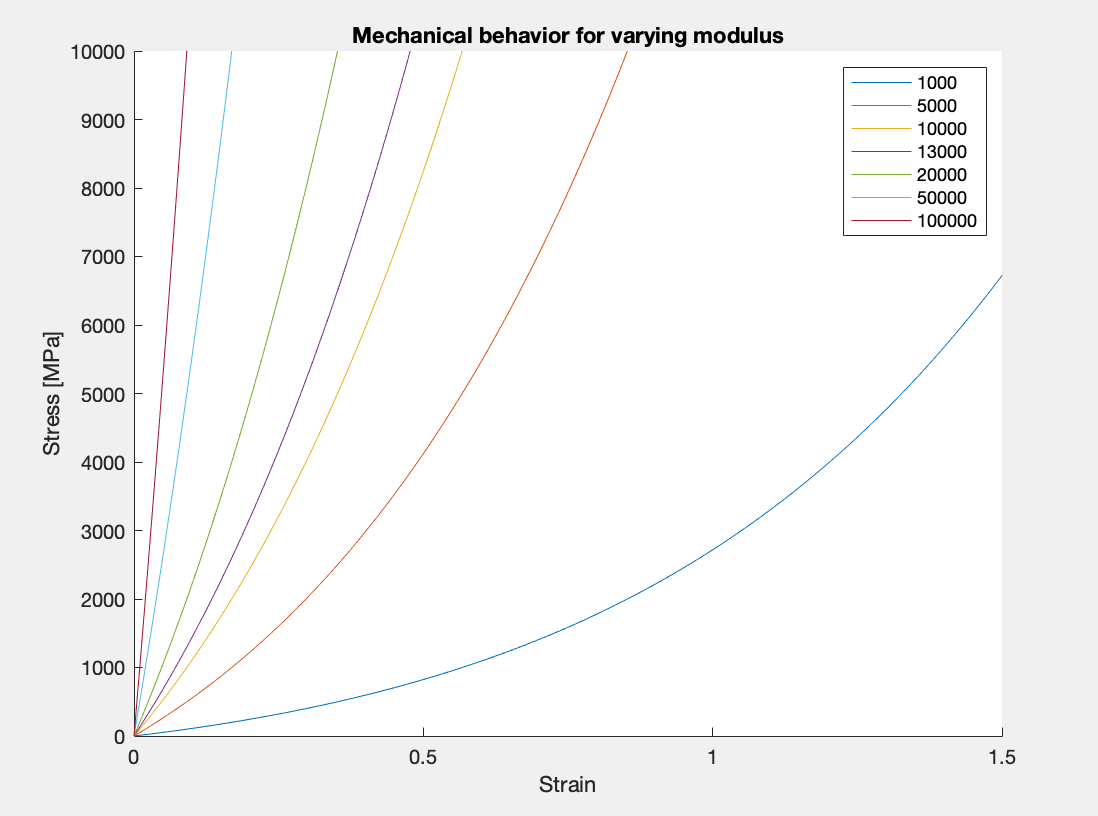
\includegraphics[width= 8cm]{nonlinear-varyingmod.png}
	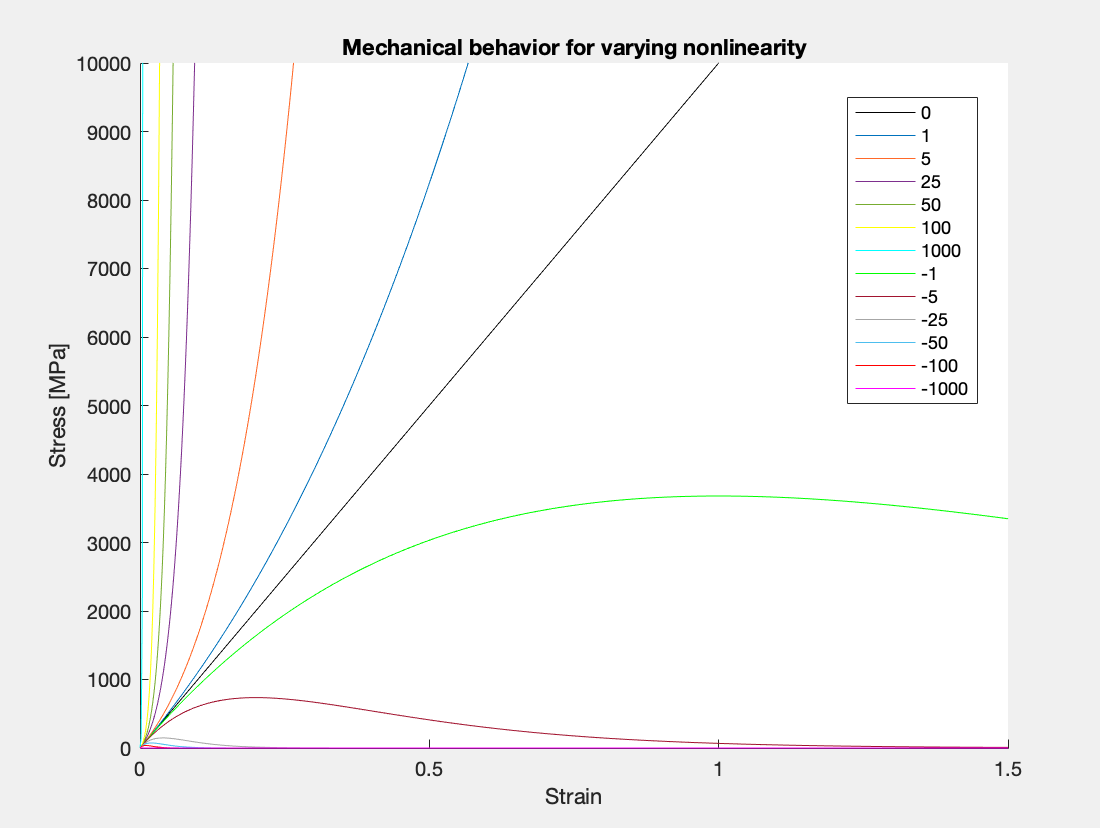
\includegraphics[width= 8cm]{modulus-varyingbeta.png}
	\caption{Family of normalized plots with varying modulus (left) and varying $\beta$ (right)}
	\end{center}
\end{figure}

\medskip 

Figure 1A clearly shows the strain range over which you see the linear and nonlinear portions of the material behavior for these materials. The blue line corresponding to $E=1000$ shows a smooth transition into the nonlinear mechanical behavior for our chosen strain range of $0<\epsilon<2$. The yellow line and dark blue lines (corresponding to $E = 10000$ and $E=100000$, respectively) see this transition occur over a smaller strain range. In Figure 1B, I explore varying the parameter $\beta$ for a constant modulus over the same strain range as in Figure 1A. By changing the magnitude of $\beta$, you can observe how different features are apparent for each curve. For example, the green line corresponding to $\beta=1$ has a clear linear region followed by the drop in stress at larger strains as expected with a negative value of $\beta$. The maroon line corresponding to $\beta=-5$ however shows a similar behavior but with these key features occurring over a shorter range of strain values.



\begin{figure}
	% make "hole" for figure: [10 text-lines tall]{on right}{this wide}
    \begin{center}
 %%   \vspace{-5mm}
%%\vspace{-20mm}		% some adjustment up or down is possible.
	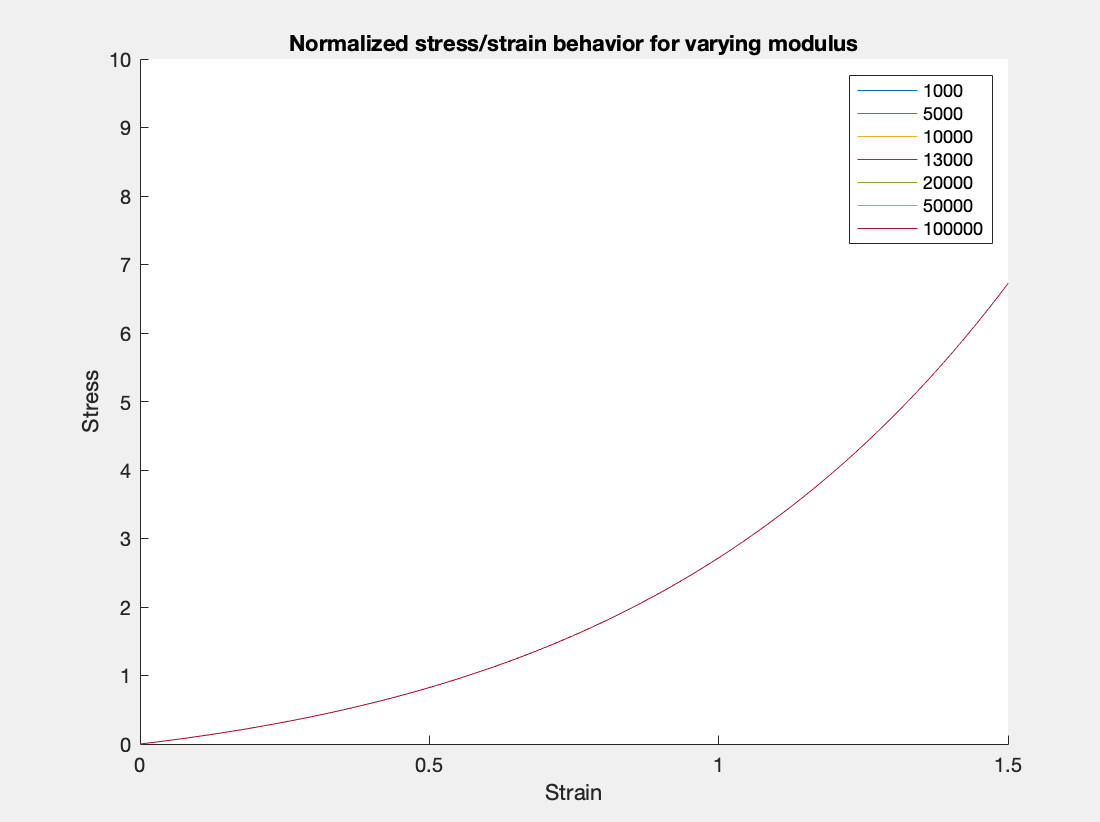
\includegraphics[width= 8cm]{normalized-pos-beta.png}
	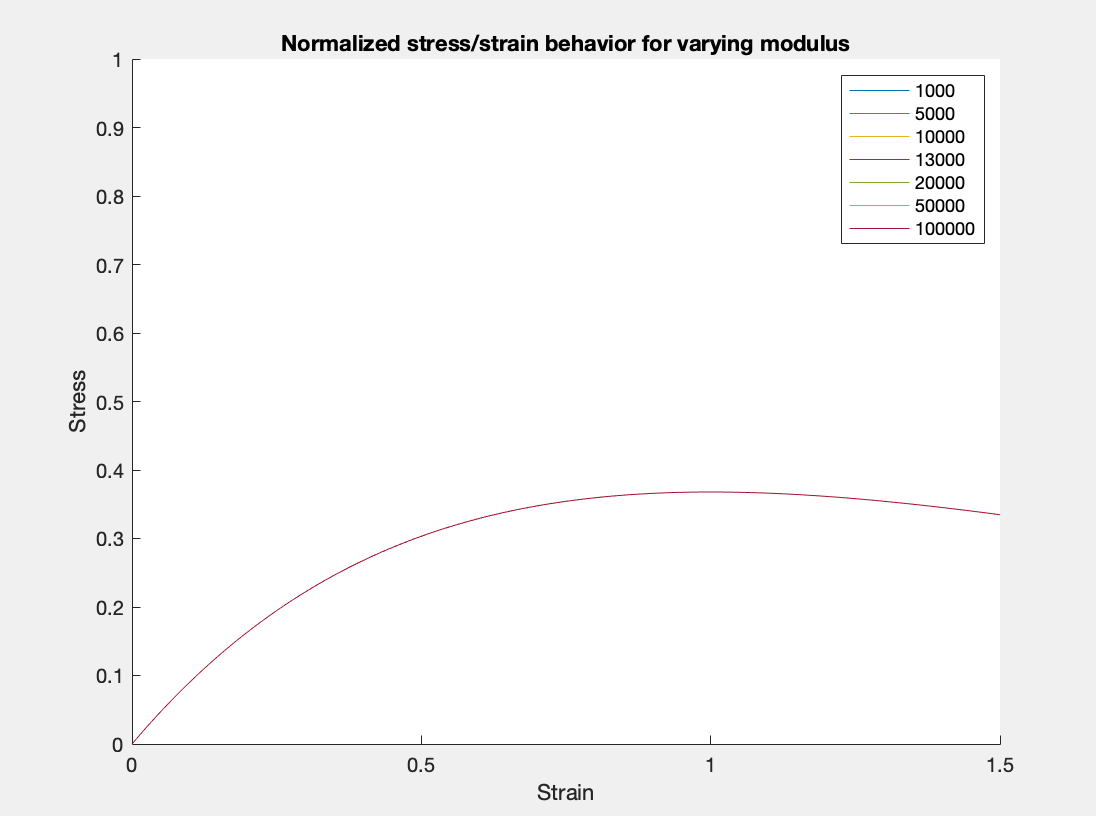
\includegraphics[width= 8cm]{normalized-neg-beta.png}
	\caption{Family of plots with varying modulus for positive $\beta$ (left) and negative $\beta$ (right)}
	\end{center}
\end{figure}

\medskip

At this point, we can pose the question: at what $\barep$ do we expect to see nonlinear behavior? Figure 3 shows a plot comparing the resolution of our overall mechanical behavior for various scales of $\beta$ for a consistent (normalized) strain range ($\barep$), as well as one that identifies the stress at which we can expect nonlinear behavior. The stress value can be determined for any defined Young's modulus and $\beta$. These graphs reinforce the ideas discussed in the previous paragraphs: (1) Scaling the stress and strain enables us to see key features of the mechanical behavior of materials that  the same overall mechanical behavior described by the defined constitutive relationship; (2) For arbitrary $E$ and $\beta$, adjusting the strain range plotted will show different features of interest; (3) The strain and stress values for any particular specific point of the plot (such as the $\barep$ at which nonlinear behavior occurs) can be computed for any arbitrary material in terms of its $E$ and $\beta$ (i.e. finding the $\epsilon$ at which this specific material with given modulus and nonlinearity can be expected to behave nonlinearly). 


\begin{figure}
	% make "hole" for figure: [10 text-lines tall]{on right}{this wide}
    \begin{center}
 %%   \vspace{-5mm}
%%\vspace{-20mm}		% some adjustment up or down is possible.
	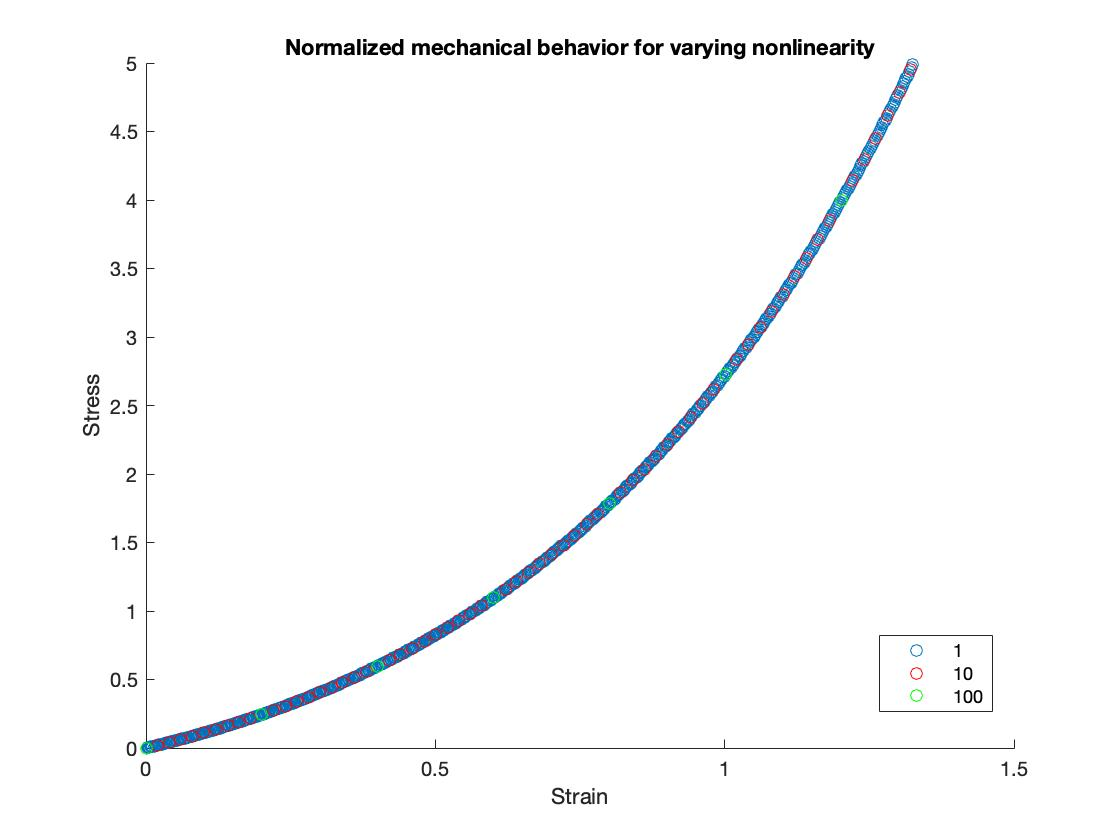
\includegraphics[width= 12cm]{beta-scaling.jpg}
	%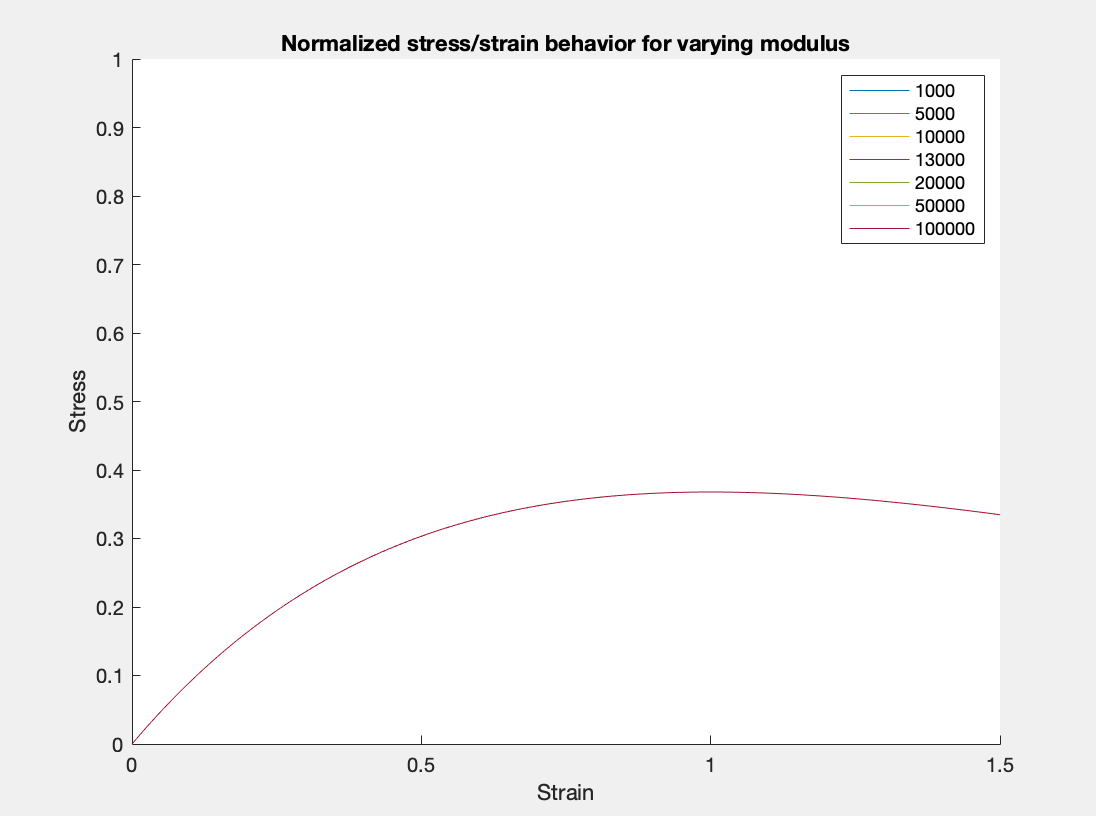
\includegraphics[width= 8cm]{normalized-neg-beta.png}
	\caption{Normalized stress/strain with increasing orders of magnitude for $\beta$}
	\end{center}
\end{figure}

\medskip

Figure 3 shows the data points for three stress/strain curves that have been normalized as described in (138). As expected, when plotting this relationship there is no dependency on $E$ or $\beta$ and therefore the curves are identical. We can see a more interesting effect, however, if our stress and strain fields are computed for a given $\beta$ and then the $\barsig$ and $\barep$ are calculated. Then we see that the \emph{resolution} of the plot is affected as function of $\beta$. More precisely, specific regions of our plot (as determined by the specified $\barep$) are more evident as a function of the prescribed $\beta$.



%%%% YOU CAN IGNORE THESE BITS: 
%A bit of notation.  We will here use square brackets to denote the dimensions of a quantity.  
%For example, if $P$ is a force and $d$ is a distance, then we might write: 
%\beq
%[P d] = F\times L = W. 
%\eeq
%This reads: 
%\begin{quote}
%	``The dimensions of $P \times d$ are force times length, which is equal to work."
%\end{quote}
%We note that dimensions are different from units in the same way that money is 
%different from dollars.  
%
%When considering the dimensions of the variables and parameters in equation (\ref{50.2}), 
%we see that the different variables and parameters have the following dimensions: 
%\bea
%\sigma &=& \frac{\mbox{force}}{\mbox{area}} = \frac{F}{L^2}  \\ 
%E &=& \frac{\mbox{force}}{\mbox{area}} = \frac{F}{L^2}  \\ 
%\ep &=& \mbox{dimensionless} = 1 \\ 
%\beta &=& \mbox{dimensionless} = 1 
%\eea
\section{Exposing the structure of our formulation to make it easier to go to $3D$}
\subsection{Weak form}
The nonlinear weak form (\ref{nlweak}) can be written: 
\beq
\int_0^L \left[
\sigma\left( \epsilon \right)
\frac{dv}{dx} - 
f(x) \cdot v(x)
\right] dx - \sigo \cdot v(L) = 0
\plabel{nlweak2}
\eeq
or 
\beq
\int_0^L \left[
\sigma\left( \frac{du}{dx} \right)
\frac{dv}{dx} - 
f(x) \cdot v(x)
\right] dx - \sigo \cdot v(L) = 0
\plabel{nlweak3}
\eeq
\subsection{Newton iteration:}
Letting $u\leftarrow u + \delta u$: 
\bea
\int_0^L \left[
\sigma\left( 
\frac{du}{dx} 
+ \frac{d\delta u}{dx} 
\right)
\frac{dv}{dx} 
\right] dx  
&=& 
\int_0^L \left[
\sigma\left( 
\frac{du}{dx} 
\right)
\frac{dv}{dx} 
\right] dx  
\nonumber \\ 
&& + 
\int_0^L \left[
\frac{d \sigma}{d\epsilon}
\left( 
\frac{du}{dx} 
\right)
 \times \frac{d\delta u}{dx} 
\frac{dv}{dx} 
\right] dx  
\plabel{200}  \\ 
&=& 
\int_0^L \left[
\sigma\left( 
\frac{du}{dx} 
\right)
\frac{dv}{dx} 
\right] dx  
\nonumber \\ 
&& + 
\int_0^L \left[
 E^* \times \frac{d\delta u}{dx} 
\frac{dv}{dx} 
\right] dx  
\plabel{201}  \\ 
\mbox{where} \qquad 
 E^* 
&=& 
\frac{d \sigma}{d\epsilon}
\left( 
\frac{du}{dx} 
\right)
\plabel{202}  \\ 
&=& \mbox{tangent\ modulus}
\eea
\subsection{Extending to multi-dimensions}
\begin{itemize}
\item 
$\int_0^L \, dx \leftarrow \int_V \, dV$. 
\item 
$ \sigma \leftarrow \sigma_{ij}$.
\item 
$ \epsilon \leftarrow \epsilon_{ij}$.
\item 
$ \frac{d v}{d x} \leftarrow \frac{\partial v_{i}}{\partial x_{j}} $. 
\item 
$ 2 \bep = \nabla \u + (\nabla \u)^T$. 
\item 
$ 2 \epsilon_{ij}  = \frac{\partial u_{i}}{\partial x_{j}} + \frac{\partial u_{j}}{\partial x_{i}}. $
\item 
$ \frac{d \sigma}{d\epsilon} \leftarrow 
\frac{\partial \sigma_{ij}}{\partial\epsilon_{kl}} $. 
\item 
$u \approx u^h = \sum_{A} d_A N_A(x)$ becomes 
$u_i \approx u_i^h = \sum_{A} d_{iA} N_A(x)$. 
\end{itemize}
\subsection{Weak form in multiple dimensions} 
\begin{tcolorbox}[title= Nonlinear Weak Form]{
% \fbox{
Given $u_{oi}$, $T_i$, the function $\sigma(\epsilon)$,  and $f_i(x)$,  
find $u^* \in \cS$ such that for all $v(x) \in \cV$, 
\beq
\int_V
\left[
\sigma_{ij}\left( \bep
\right)
\frac{\partial v_i}{\partial x_j} - 
f_i(x) v_i(x)
\right] dV - 
\int_{\Gamma_T} 
T_i \cdot v_i \,  dS
= 0
\plabel{3Dweak}
\eeq
where
\bea
\cS &=& \left\{ \u(x) | \u(x)\in C^0[V];\  u_i|_{\Gamma_u} = u_{oi}. \right\}
\plabel{S3} \\ 
\cV &=& \left\{ \v(x) | \v(x)\in C^0[V];\  v_i|_{\Gamma_u} = 0. \right\}
\plabel{V3}
\eea
}
\end{tcolorbox}
\subsection{A sample $3D$ constitutive equation} 
The classical form of the linear elastic isotropic constititive equation in 
$3D$ is: 
\beq
\ep_{ij} = \frac{1+\nu}{E} \sigma_{ij} 
			- \frac{\nu}{E} \delta_{ij} \sigma_{kk}. 
			\plabel{e-nu}
\eeq
When expressing stress in terms of strain, the Lam\' e parameters, 
$\lambda, \mu$, are often used as material properties.  In terms of the
Lam\' e parameters, we may write the stress-strain relation as: 
\beq
\sigma_{ij} = \lambda \delta_{ij} \ep_{kk} + 2\mu \ep_{ij}. 
			\plabel{lam-mu}
\eeq
\begin{tcolorbox}[title= Exercise]{  
	\begin{enumerate}
		\item Look up relation between $E,\nu, \lambda, \mu\equiv G, K, M$ at
			\href{https://en.wikipedia.org/wiki/Elastic_modulus}{label}
			% \href{https://en.wikipedia.org/wiki/Elastic_modulus}{https://en.wikipedia.org/wiki/Elastic_modulus}
		\item Use (\ref{lam-mu}) and (\ref{e-nu}) to derive 
			the expression for $\mu$ in terms of $E$ and $\nu$, 
			and also for $E$ in terms of $\lambda$ and $\mu$.  
		\item Derive (\ref{deltaV}). 
	\end{enumerate}
	}
\end{tcolorbox}

In general, strain can be decomposed into two parts: volume change and shape 
change.  For large deformation, that decomposition is a multiplicative 
decomposition of the deformation gradient.  For small (linearized) 
deformations, the decomposition simplifies to an additive decomposition.  
First recall that for small strains, the volume change per unit volume 
is: 
\beq
\frac{\Delta V}{V} \equiv \Delta = \ep_{kk}
\plabel{deltaV}
\eeq
Now we introduce the deviatoric strain, $e_{ij}$, so that: 
\beq
\ep_{ij} = \frac{\Delta}{3} \delta_{ij} + e_{ij} . 
\plabel{dev-def}
\eeq
In a similar way, we can introduce the deviatoric stress $s_{ij}$ and 
pressure $p$, so that: 
\bea
\sigma_{ij} &=& -p \delta_{ij} + s_{ij} 
 \\ 
 p &=& - \frac{1}{3} \sigma_{kk} 
\eea
One way to think about why an isotropic material has two different material 
properties is that it has one ``spring" constant associated with volume change, 
and a different one associated with shape change.  Therefore: 
\bea
 p &=& -K \Delta \\ 
 \bs &=& 2\mu \be = 2G \be
\eea
\end{document}
